\documentclass{article}
\usepackage[sglblindworkshop, final]{neurips_2026}
\workshoptitle{Predictive AI Evaluation Competition (PAIEC)}
\usepackage[utf8]{inputenc}
\usepackage[T1]{fontenc}
\usepackage{hyperref,url,booktabs,amsfonts,amsmath,amssymb,nicefrac,microtype,xcolor,graphicx,pifont}
\hypersetup{colorlinks=true,linkcolor=blue!50!black,citecolor=blue!50!black,urlcolor=blue!50!black}
\newcommand{\ch}[1]{\ding{\numexpr171+#1\relax}}

\title{Predicting AI Results on New Benchmarks\\with a Gaussian Process IRT Model Fit at Test Time}
\author{%
  Uriel Nguefack Yefou\\
  Concordia University\\
  Team \emph{Pooled Priors}\\
  \texttt{uriel.nguefackyefou@mail.concordia.ca}
}

\begin{document}
\maketitle

\begin{abstract}
Running every AI system on every benchmark is costly, so it is useful to predict how a system will do on a new
benchmark from only a few of its results. The Predictive AI Evaluation Competition (PAIEC) asks for a predictor that
estimates whether a system answers an item correctly, when the benchmark is not in the training data and labels are
revealed a few at a time (0, 1, 3, 7, 15 and 31 per system and benchmark). This is challenging because, with so few
labels, most of the error comes from not knowing how well the system does on the benchmark as a whole. To address
this challenge, we design GP-IRT, a solution that fits a logistic item response model on each test benchmark at test
time, using the labels of all systems on that benchmark. Item effects have a Gaussian process prior over item
embeddings, so items with similar text get similar difficulty, and predictions are averaged over a grid of prior
scales with weights from the Laplace marginal likelihood. Specifically, the prior on the benchmark level is centred on
the accuracy of groups of the size used at test time, which is near 0.36 in training and 0.35 in the test groups we
recovered from formative feedback. We evaluate GP-IRT with a simulator of the official protocol on held-out
benchmarks. The results show that GP-IRT achieves a Brier ALC of 0.1797, against 0.1869 for a group mean and 0.25
for a constant 0.5. Centring the prior gives the largest single gain: it lowers the Brier score at budget 0 from 0.248
to 0.236 and the Brier ALC by 0.002.
\end{abstract}

\section{Introduction}
Benchmarks are the main tool to compare AI systems, but running a new system on a large set of benchmarks takes time
and money. Predictive evaluation aims to estimate the result of a system on an item before running it, using results
that are already known~\citep{paiec2026}. PAIEC studies this question in a hard setting: the test benchmarks never
appear in training, and the predictor only sees a handful of labels on each of them. The training pool is the AI
Measurement Data Bank~\citep{measurementdb2026}, and predictions are scored with the Brier score~\citep{glenn1950verification}
averaged over label budgets.

\textbf{Limitation of existing solutions:} Item response theory (IRT)~\citep{lord2012applications} models the
probability of a correct answer from the ability of a subject and the difficulty of an item, and it has been used to
evaluate language models from a few items. For example, tinyBenchmarks~\citep{polo2024tinybenchmarks} estimates the
accuracy of a new model from a small set of items, using item parameters learned from many models already evaluated
on the same benchmark. In PAIEC the test benchmarks are new, so item parameters are not known in advance and must be
learned at test time from the few revealed labels. Simple baselines such as the mean of the revealed labels of a group
do not use the labels of other systems or the text of the items.

\textbf{Challenges:} Working with new benchmarks and very few labels poses several challenges:
\ch{1} \emph{Unknown benchmark level:} with zero or one label, the error mostly comes from the overall level of the
system on the benchmark, and not from single items.
\ch{2} \emph{Few labels per item:} most items have no label, so their difficulty must be inferred from the labels
of other systems and from the item text.
\ch{3} \emph{Benchmarks differ a lot:} on some benchmarks items are almost always right or always wrong, while on
others the item effects are small, so a single prior does not fit all of them.
\ch{4} \emph{No test benchmark for model selection:} the formative feedback of Codabench~\citep{xu2022codabench} is
computed on a new random draw for each submission, so it cannot be used to compare models.

\textbf{Contribution:} In this paper, we make the following contributions:
\begin{itemize}\itemsep0pt
\item To address challenge \ch{1}, GP-IRT uses a prior on the benchmark shift centred on the level of training groups
of realistic size. We show from the formative logs that the test groups have the same low accuracy (0.35 on average).
\item To address challenge \ch{2}, GP-IRT pools the labels of all systems on a benchmark and gives the item effects a
Gaussian process prior~\citep{rasmussen2006gaussian}. Its kernel combines the similarity of text embeddings, of
metadata tokens, and a linear kernel on embeddings centred within the benchmark.
\item To address challenge \ch{3}, GP-IRT fits the model for a grid of prior scales and averages the predictions with
weights from the Laplace marginal likelihood, as in Bayesian model averaging~\citep{hoeting1999bayesian}.
\item To address challenge \ch{4}, we built a simulator of the official protocol with 5-fold cross-validation over
benchmarks and paired comparisons, and made every design choice with it. We release the code and the simulator.
\end{itemize}

\section{Task and Data}
\textbf{Task:} A subject is an AI system with fixed settings. An item is one task, with its text, some metadata and an
anonymous benchmark ID. A group is one subject on one benchmark. In each scored group with at least 80 items, the
items are split in two halves: labels are revealed from one half, and the other half is scored. Labels come in nested
steps of 0, 1, 3, 7, 15 and 31 per group. The predictor sees the labels of every group, including groups it is not
predicting. The score is the Brier ALC, $0.1B_0+0.2B_1+0.2B_3+0.2B_7+0.2B_{15}+0.1B_{31}$, averaged over groups.

\textbf{Training data:} We use only the public training pool \texttt{aims-foundations/measurement-db} (revision
\texttt{54074453}). We keep benchmarks with binary item-level responses and \texttt{release = public}, which gives 160
benchmarks. Of these, 92 have at least one group with 80 to 1000 items, for a total of 10{,}208 groups, 154{,}628
items and 4.3M subject and item cells. Each cell holds $n$ trials and $k$ successes. No other evaluation data is used.

\section{GP-IRT: Item Response Prediction Fit at Test Time}
\subsection{Overview}
For each test benchmark, GP-IRT works in five steps. It first collects all revealed labels on the benchmark, from any
subject (Step~1). It then builds item vectors from the item text and metadata (Step~2). It fits a logistic item
response model with a Gaussian process prior on the item effects, once for each point of a grid of prior scales
(Step~3). The predictions of the grid are averaged with weights from the Laplace marginal likelihood (Step~4).
Finally, the predictor returns the probability that the subject answers each target item correctly (Step~5). The
fits are redone each time new labels arrive, so the model adapts during the run.

\subsection{Model}
Fix a benchmark $b$ and let $\mathcal{L}$ be the labels revealed on $b$, from any subject. For subject $s$ and item
$t$,
\begin{equation}
\operatorname{logit} P(y_{st}=1) = c_t + m + a_s + d_t,\quad
a_s\sim\mathcal{N}(0,\sigma_a^2),\; d\sim\mathcal{GP}(0,\sigma_d^2 K).
\end{equation}
Here $c_t$ is a fixed offset from a prior model (Section~\ref{sec:prior}), $m$ is a shift for the benchmark, $a_s$ is
a shift for the subject, and $d_t$ is the item effect, shared by all subjects of the benchmark. The prior on $m$ is
described in Section~\ref{sec:shift}. The item kernel is
\begin{equation}
K = (1-\rho_\ell)\big[\rho\,e^{(\cos(e_i,e_j)-1)/\ell} + \rho_f\,\kappa_{\text{tok}}(i,j) + (1-\rho-\rho_f)\,\mathbb{1}[i=j]\big]
  + \rho_\ell\,\frac{\tilde e_i^\top \tilde e_j}{\overline{\|\tilde e\|^2}}.
\end{equation}
$e$ is the normalised \texttt{multilingual-e5-small}~\citep{wang2024multilingual} embedding of the item text and
metadata. $\kappa_{\text{tok}}$ is the cosine similarity of \texttt{key=value} metadata tokens, counting only tokens
that appear on at least two labeled items. $\tilde e = e-\bar e_{\mathcal{L}}$ is the embedding minus its mean over the
labeled items of the benchmark. The last term is a Bayesian linear regression of item difficulty on the embedding,
learned for each benchmark from its revealed labels.

\subsection{Inference}
We find the posterior mode with Newton's method. The Hessian block of the subject effects is diagonal, so we remove it
with a Schur complement. What is left is a block for $m$ and the labeled item effects, whose size is at most the number
of distinct labeled items. One Newton step costs $O(|\mathcal{L}| + n_s n_{\mathcal{L}} + n_{\mathcal{L}}^3)$. The
Laplace posterior~\citep[Chapter~3]{rasmussen2006gaussian} gives a mean $\mu$ and a variance $v$ of the logit for any
target item, labeled or not, through the Gaussian process conditional of $d_t$ given $d_{\mathcal{L}}$. We predict
$\sigma\big(\mu/\sqrt{1+\pi\gamma v/8}\big)$. With $\gamma=1$ this is the usual probit approximation of the predictive
integral~\citep{mackay1992evidence}. We use $\gamma=0.35$ while the target subject has at most three labels on the
benchmark and $\gamma=0.2$ after that, values chosen in simulation (Section~\ref{sec:risk}). We checked the code against
a dense Laplace solver, and both agree to machine precision.

\subsection{Averaging over Prior Scales}
We fit the model for every combination of $\sigma_a\in\{0.4,0.8,1.6\}$, $\sigma_d\in\{0.8,1.6,3.2\}$ and the three
components of the shift prior below, with $\rho=0.73$, $\rho_f=0.17$, $\ell=0.12$ and $\rho_\ell=0.4$. The predicted
probabilities are averaged with weights proportional to the Laplace marginal likelihood. This is done for each
benchmark and each set of revealed labels separately.

\subsection{Prior on the Benchmark Shift}\label{sec:shift}
The shift $m$ sets the overall level of a subject on a new benchmark. Its prior is a mixture with equal weights,
\begin{equation}
m \sim \tfrac13\big[\mathcal{N}(\mu_0, 0.8^2) + \mathcal{N}(\mu_0, 1.6^2) + \mathcal{N}(\mu_0, 3.2^2)\big],
\qquad \mu_0=-0.6,
\end{equation}
and each component is one more axis of the averaging grid. The wide component allows the model to follow benchmarks
where a subject gets almost everything right or wrong, while the narrow one keeps predictions stable with one or two
labels. The centre $\mu_0$ matters more than the scales. In the training groups of realistic size, the mean logit
accuracy is $-0.87$ with a standard deviation of 1.8, so a prior centred at zero starts every new benchmark from an
accuracy that is too high. We set $\mu_0$ by cross-validation (Section~\ref{sec:results}). The selected value lies
between zero and the training mean, because part of the low level is already carried by the offset $c_t$, whose mean
is negative, and the probit correction pulls predictions toward 0.5.

\subsection{Prior across Benchmarks and Second Model}\label{sec:prior}
We take hidden states of Qwen2.5-7B-Instruct~\citep{qwen2025qwen25technicalreport} (layer 21 of 28, mean over tokens,
standardised) and fit a ridge regression to the mean logit accuracy of each item, with equal weight for all training
benchmarks. The output is $z_t$, and we set $c_t = 0.3\,z_t$. With no labels, the prediction is the prior predictive,
averaged over the components of the shift prior. The final predictor is the average of two copies of the model that
differ only in the item vectors used by the kernel: e5-small embeddings in one, and Qwen hidden states in the other.

\subsection{Implementation}
We keep the platform's default random choice of labels (Section~\ref{sec:negative}). Each prediction worker caches one
fit per benchmark and set of labels. Since the label list only grows, an unchanged set is detected from its length and
last entry. Item vectors are cached too. Without a GPU, or if Qwen cannot be loaded, the predictor uses the e5 model
alone with no offset $c_t$. If Qwen fails during the run, it is switched off and the run continues with the e5 model.
In simulation, the e5 model alone is worse by only 0.0003 ALC in the realistic setting. A prediction takes 15 to
110~ms on the A100 we used for testing.

\section{Experimental Setup}\label{sec:sim}
We built GP-IRT in Python. The hidden states were computed on one A100 80GB GPU (about 2.5 hours), and the simulations
ran on 30 CPU cores, where one setting of 1000 episodes takes 10 to 20 minutes in the realistic setting.

\textbf{Simulator:} Test benchmarks never appear in training, so every choice was made with a simulator of the official
protocol and 5-fold cross-validation over benchmarks. Groups are added to a draw one at a time. Groups whose benchmark
or model name is already in the draw come last, and ties are broken at random. We stop when the draw would pass 1000
subject and item pairs. In each group, the distinct items are split at random, with the odd item going to the label
pool. Labels come in random order, one sampled trial per item, and every group sees the labels of all other groups.

\textbf{Settings:} We use three settings. In the realistic setting, our main one, only groups with at most 200 items
are allowed. A draw then has on average 6.9 groups, 5.9 benchmarks and 142 items per group. The large group setting
allows all groups with 80 to 1000 items and gives about 3 groups per draw. In the many subjects setting, the limit
counts distinct items, so a benchmark can have hundreds of subjects.

\textbf{Baselines:} We compare GP-IRT with a constant 0.5, the mean of the revealed labels of the group with a
Beta(1,1) prior, and the Bayes predictor of the group accuracy from the group's own labels, with the accuracies of
training groups from other folds as its prior (groups of 80 to 200 items, in all three columns). We also compare with
IRT models without item effects and with independent item effects.

\textbf{Metrics:} We compute the exact Brier score of each group over all response rows, apply the ALC weights, and
average over groups and then over episodes. Two models are always compared on the same episodes, with the same splits
and the same labels, and we report paired mean differences with their standard errors. Settings were chosen on one
seed and checked again on episodes drawn with another.

\textbf{Formative feedback:} Each Codabench submission is scored on a new draw of about nine groups, and the scoring
log gives the Brier score and the calibration error (ECE) of every group at every budget. These logs say little about
which model is better, since the draws change. However, they describe the test groups. A draw has about nine groups
from seven benchmarks, with 88 to 152 items per group, which is what the realistic setting produces. The logs also
give the accuracy of each group. Our first three submissions predicted exactly 0.5 at budget 0, and in that case the
ECE of a group is $|q-0.5|$, where $q$ is its accuracy. Later submissions predicted slightly below 0.5 at budget 0, so
their Brier score is above 0.25 only when $q>0.5$, which gives the side. On the 27 groups recovered in this way, the
mean accuracy is 0.35. Fig.~\ref{fig:acc} compares them with the training groups. The test groups look like the
training groups of realistic size (mean 0.36 per group, 0.39 per benchmark), and not like the training pool as a whole
(0.49 per benchmark), where large benchmarks with many subjects weigh the most. The logs pointed us to the realistic
setting and to the level of the shift prior. The value of every parameter, including the centre of that prior, was
then chosen by cross-validation on the training pool.

\begin{figure}[t]
\centering
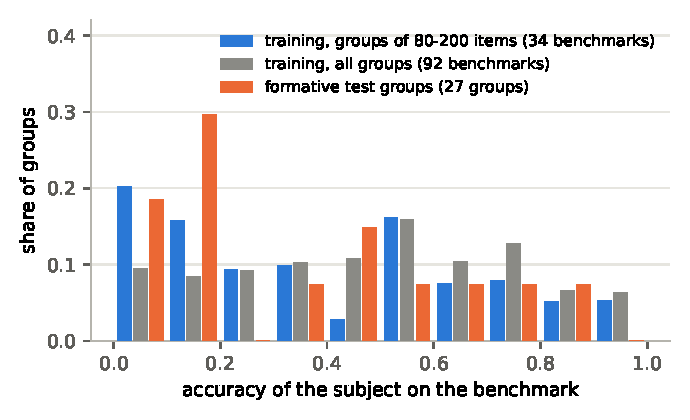
\includegraphics[width=0.6\linewidth]{group_accuracy.pdf}
\caption{Accuracy of a subject on a benchmark, for training groups and for test groups seen in formative feedback.}
\label{fig:acc}
\end{figure}

\section{Evaluation Results}\label{sec:results}
We evaluate GP-IRT through four research questions (RQs): (1) we assess how accurately GP-IRT predicts results on new
benchmarks compared with the baselines; (2) we study the contribution of each component; (3) we analyze the effect of
the prior on the benchmark shift; and (4) we examine the risk of bad predictions with very few labels.

\begin{table}[t]
\centering\small
\caption{Simulated Brier scores with held-out benchmarks (1000 episodes per setting, the same in every row).}
\label{tab:main}
\setlength{\tabcolsep}{3pt}
\begin{tabular}{lccccccc|cc}
\toprule
& \multicolumn{7}{c|}{realistic} & large & many \\
Model & $B_0$ & $B_1$ & $B_3$ & $B_7$ & $B_{15}$ & $B_{31}$ & ALC & ALC & ALC \\
\midrule
Constant 0.5 & .2500 & .2500 & .2500 & .2500 & .2500 & .2500 & .2500 & .2500 & .2500 \\
Group mean, Beta(1,1) & .2500 & .2121 & .1862 & .1708 & .1619 & .1572 & .1869 & .2083 & .2133 \\
Bayes, own labels, empirical prior & .2356 & .2072 & .1856 & .1715 & .1626 & .1576 & .1847 & .2089 & .2129 \\
IRT, no item effects & .2500 & .2077 & .1835 & .1698 & .1616 & .1571 & .1852 & .2096 & .2047 \\
IRT, independent item effects & .2500 & .2113 & .1883 & .1741 & .1652 & .1599 & .1888 & .2091 & .1799 \\
GP-IRT, e5 RBF kernel & .2500 & .2083 & .1846 & .1700 & .1605 & .1540 & .1851 & .2075 & .1738 \\
\quad + metadata token kernel & .2500 & .2090 & .1839 & .1684 & .1583 & .1510 & .1840 & .2071 & .1728 \\
\quad + linear kernel, centred emb. & .2500 & .2091 & .1856 & .1688 & .1582 & .1507 & .1844 & .2046 & .1726 \\
\quad + Qwen offset $c_t$ & .2483 & .2082 & .1851 & .1685 & .1580 & .1507 & .1839 & .2041 & .1729 \\
\quad + second model, Qwen kernel & .2483 & .2083 & .1852 & .1684 & .1578 & .1502 & .1838 & .2039 & .1709 \\
\quad + retuned scales and $\gamma$ & .2483 & .2055 & .1829 & .1672 & .1571 & .1497 & .1824 & .2038 & .1701 \\
\quad + shift scale mixture, $\gamma$ by labels & .2483 & .2046 & .1822 & .1668 & .1568 & .1494 & .1819 & .2046 & .1698 \\
\quad + shift prior centred at $-0.6$ (final) & \textbf{.2356} & \textbf{.2012} & \textbf{.1814} & \textbf{.1666} & \textbf{.1567} & \textbf{.1494} & \textbf{.1797} & .2041 & \textbf{.1693} \\
\bottomrule
\end{tabular}
\end{table}

\textbf{RQ1: How accurately does GP-IRT predict results on new benchmarks compared with the baselines?:}
Table~\ref{tab:main} shows the Brier scores of GP-IRT and the baselines. GP-IRT achieves the lowest ALC in the
realistic and many subjects settings (0.1797 and 0.1693), against 0.1869 and 0.2133 for the group mean. With large
groups, it is within 0.0003 of the best row, which is inside the noise of that setting. The Bayes reference is a useful
point of comparison. At budget 0 it predicts the mean training accuracy, which is the best constant under the training
distribution. Its $B_0$ is 0.2356, and GP-IRT reaches the same value, so little is left to gain at budget 0 without
information on single items. From budget 1 on, GP-IRT is better than this reference by 0.004 to 0.008 at every budget.
This gain comes from the labels of other subjects on the same benchmark and from the item kernel. Fig.~\ref{fig:curves}
shows the curves.
Two oracles bound what a predictor can reach in the realistic setting. If the accuracy of each group were known, a
constant prediction per group would score 0.1503. If the accuracy of each item for each subject were known, the Brier
score would be 0.011. Our $B_{31}$ of 0.1494 is just below the first oracle. With 31 labels, the model knows the group
level well and gets a little more from the items, but the gap to the second oracle shows how much of the item signal
stays out of reach.
On Codabench, the final model (submission 1018959) scored 0.182 Brier ALC, with an ECE of 0.139. Our seven earlier
submissions scored between 0.164 and 0.228. Each submission is scored on a new draw of eight or nine groups, so these
numbers move by several hundredths from one draw to the next, and we did not use them to rank models.

\begin{figure}[t]
\centering
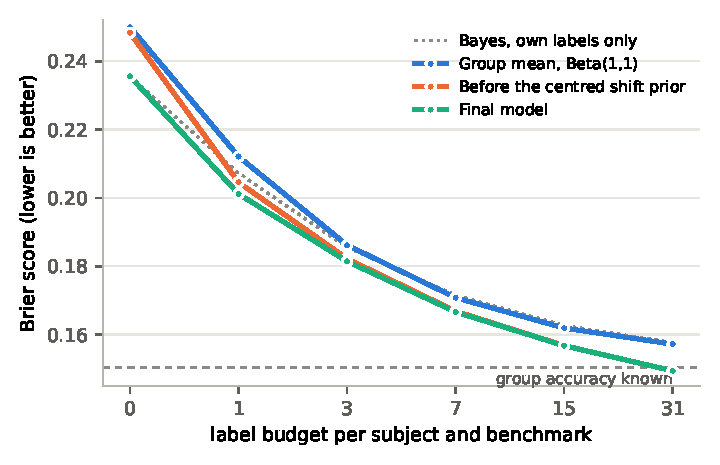
\includegraphics[width=0.62\linewidth]{learning_curves.pdf}
\caption{Brier score by budget in the realistic setting.}
\label{fig:curves}
\end{figure}

\textbf{RQ2: What is the contribution of each component?:} Table~\ref{tab:main} adds the parts of the model one at a
time, on the same 1000 episodes in every row. The paired standard error of the difference between two rows is about
$10^{-4}$ in the realistic setting. The centred shift prior gives the largest step in the realistic setting
($-0.0022$, from 0.1819 to 0.1797), almost all of it at budgets 0 and 1. The centred linear kernel gives the largest
step with large groups ($-0.0025$) and helps from budget 7 on. Most of the other rows move the ALC by less than 0.001.

\textbf{RQ3: How does the prior on the benchmark shift affect the results?:} We compared centres and scales on 300
paired episodes of the realistic setting, against the model of the previous row of Table~\ref{tab:main}. Centres of
$-0.4$, $-0.6$ and $-0.8$ lower the ALC by 0.0018 to 0.0022, all with a standard error near 0.0002, while $-1.2$ gives
only 0.0010. The scales matter less: $(1, 2, 4)$, $(0.8, 1.6, 3.2)$ and $(1.5, 3)$ are within 0.0001 of each other.
Gaussian mixtures with two or three components fit directly to the training group accuracies did about as well
($-0.0023$), so we kept the simpler prior. Raising the weight of the Qwen offset to 0.5 or making predictions more
confident with few labels did not add to the gain. Once the prior is centred, the Qwen offset itself no longer matters:
setting $c_t=0$ changes the ALC by $+0.00001\pm0.00007$. We kept it, since the runtime was checked end to end with it.
On 1000 new episodes drawn with another seed, the final model is better than the previous row by $0.0022\pm0.0001$
ALC, of which 0.012 at budget 0 and 0.004 at budget 1. In the large group setting, where the training accuracy is
higher, the centred prior neither helps nor hurts: the change is $-0.0008\pm0.0005$ on the episodes used for the
choice and $+0.0002\pm0.0003$ on new episodes.

\textbf{RQ4: How risky are predictions with very few labels?:}\label{sec:risk} With one to three labels, a predictor can
move away from the truth. In simulation, $B_3>B_0$ happens for about a quarter of the groups, and in the 53 groups of
our first formative logs it happened for 24.5\%, so the simulator matches the real behaviour on this point. A smaller
variance scale $\gamma$ makes predictions more confident. It lowers the mean ALC down to about $\gamma=0.1$, but it also
makes bad groups more common: the share of groups with $B_3>0.3$ grows from 5.2\% at $\gamma=0.5$ to 7.4\% at
$\gamma=0.2$. We kept $\gamma=0.35$ while the subject has at most three labels, and $\gamma=0.2$ after that, when the
posterior is better informed.

\section{Discussion}\label{sec:negative}
While GP-IRT improves over the baselines in our simulation, it holds certain limitations:

\textbf{Simulator assumptions:} The simulator depends on how we read the draw rule. We matched it to the formative
logs, and we checked every choice in three settings for this reason.

\textbf{Level of the test groups:} The centred shift prior helps because test groups have a low accuracy on average,
as in the training groups of the same size. On a test set dominated by easy benchmarks, it would give back part of its
gain at budget 0, although it did not hurt in our large group setting.

\textbf{Model assumptions:} The model assumes that item effects are the same for all subjects of a benchmark, apart
from the logistic link. With no labels, it predicts close to the average level of a group, since the accuracy of a
subject on a new benchmark is hard to predict from the data we have. The Qwen parts need a GPU at test time; without
one, the predictor still runs with the e5 model alone.

\textbf{Approaches that did not help:} We tested the following ideas with the same paired simulation and dropped them.
\begin{itemize}\itemsep0pt
\item Predicting budget 0 from item text and subject attributes with LightGBM~\citep{ke2017lightgbm} (e5 embeddings,
text statistics, provider, release date, size, model name). The best $B_0$ was 0.248, against 0.250. Once the shift
prior is centred, the model already reaches the $B_0$ of the Bayes reference (0.2356).
\item Asking Qwen2.5-7B to rate item difficulty from 1 to 9. The rank correlation with measured difficulty inside a
benchmark was $-0.03$. Item contents rarely include a reference answer (3 benchmarks out of 92), so we could not score
the likelihood of the correct answer either.
\item Looking for the same item in other benchmarks. Fewer than 0.1\% of items have a match with cosine above 0.95.
\item Learning a projection of the embeddings for the kernel by maximising the marginal likelihood on training groups.
It was worse on held-out benchmarks, and a learned low-rank metric for the linear kernel did not help either.
\item Bigger item vectors (e5-base, e5-large, Qwen2.5-7B layers 14, 21 or 28) as the only kernel input. None beat
e5-small: with so few labels, the number of labels limits the model more than the quality of the vectors. Qwen2.5-14B
in place of the 7B model gained 0.0002 ALC for twice the memory.
\item Stacking with LightGBM on model outputs and label counts, and Platt scaling~\citep{platt2000probabilities} per
budget. Both were worse on held-out benchmarks, because calibration learned on some benchmarks does not carry over to
others.
\item Other label choices: uncertainty, overlap with other subjects, embedding diversity, D-optimal design. No
significant difference from random order.
\item Learning the centre of the shift prior during the run, from the label rates of the other benchmarks in the same
draw (a hierarchical prior with a shared centre). It was worse in every fold, by 0.0001 to 0.0007 ALC depending on the
prior width of the centre, even in the fold whose benchmarks are hardest. The level of a subject on one benchmark tells
little about the level of other subjects on other benchmarks.
\item Weights for the averaging grid learned on training benchmarks. The posterior over the grid stays almost flat even
with 31 labels (weights from 0.026 to 0.048 over 27 points), so a learned prior is close to the uniform one.
\item A prior on subject ability from the same model name on other benchmarks. The out-of-fold correlation with
ability on held-out benchmarks was $-0.16$, and there was no gain. A ridge regression of the group level on all subject
metadata tokens did no better: its out-of-fold correlation with the group logit was between $-0.19$ and $+0.24$
depending on the subset, and on all groups it was worse than a constant. A prior on item difficulty inside a benchmark
from a ridge on centred Qwen states (Spearman 0.07) hurt $B_0$ and $B_1$ more than it helped later.
\item Numeric metadata (lengths, counts and similar fields) or text statistics as an extra kernel term. All versions
were 0.0001 to 0.0005 worse.
\end{itemize}

\section{Related Work}
\textbf{Item response theory:} IRT~\citep{lord2012applications} models a correct answer from the ability of a subject
and the difficulty of an item. tinyBenchmarks~\citep{polo2024tinybenchmarks} uses IRT to estimate the accuracy of a
language model from a small set of items, with item parameters learned from models already evaluated on the same
benchmark. GP-IRT instead learns the item effects of a new benchmark at test time, and shares information between
items through a Gaussian process prior on their embeddings.

\textbf{Gaussian process classification:} GP-IRT uses the Laplace approximation for Gaussian process
classification~\citep{rasmussen2006gaussian} and the probit approximation of the predictive
integral~\citep{mackay1992evidence}. Averaging predictions over prior scales with weights from the marginal likelihood
follows Bayesian model averaging~\citep{hoeting1999bayesian}.

\section{Conclusion}
In this paper, we designed GP-IRT, a solution for predicting whether an AI system answers an item of a new benchmark
correctly from a few revealed labels. GP-IRT fits a logistic item response model on each benchmark at test time, pools
the labels of all subjects, shares information between items through a Gaussian process prior on their embeddings,
and averages over prior scales. Experiments with a simulator of the official protocol on held-out benchmarks showed
that GP-IRT achieves a Brier ALC of 0.1797, and that centring the prior on the benchmark level is the largest single
gain. The remaining error is mostly at the level of the group, which is hard to predict for a new benchmark from the
data we have.

\textbf{Reproducibility:}\sloppy{} The code is available at \url{https://github.com/nguefackuriel/paiec-gpirt}. The
README describes the full pipeline: download of the training pool, the tables, the benchmark folds, the embeddings,
the simulator (\texttt{paiec/sim.py}), every experiment script (\texttt{scripts/try\_*.py},
\texttt{scripts/final\_table.py}), the Qwen prior (\texttt{scripts/llm\_embed.py},
\texttt{scripts/build\_qwen\_prior.py}), the check that the submission matches the simulator
(\texttt{scripts/parity\_v8.py}) and packaging. The recovery of test group accuracies from formative logs is in
\texttt{scripts/formative\_acc.py}. Pretrained models: \texttt{intfloat/multilingual-e5-small} and
\texttt{Qwen/Qwen2.5-7B-Instruct}. Training data: only \texttt{aims-foundations/measurement-db}.

\textbf{Use of AI assistants:} The code, the experiments and drafts of this report were made with the help of an LLM
coding assistant (Claude Code, Anthropic). All results come from the code in the repository.

{\small
\bibliographystyle{plainnat}
\bibliography{references}
}

\end{document}
